% Say Yes to the Guess:
% Finalish revisions 10.Feb. 2013



%\documentclass[pdftex,12pt,fullpage,oneside,endnotes]{amsart}
\documentclass[12pt,fullpage,endnotes]{article}
%\usepackage{apsr}
\usepackage{array,amsmath,psfrag,amssymb,subfigure,tabularx}
\usepackage{multicol}
\usepackage{booktabs}
\usepackage[usenames]{color}
\usepackage{datetime}
\usepackage{dcolumn}
\usepackage{wrapfig}
\usepackage{setspace}
\usepackage{url}
\usepackage[english]{babel}
\usepackage{times}
\usepackage{multirow}
\usepackage[pdftex]{graphicx}
\usepackage{epstopdf}
\usepackage{lscape}
\usepackage{array}
\usepackage{booktabs}
\usepackage{endnotes}
\usepackage{rotating}

%\usepackage[nolist]{endfloat}


\usepackage{footmisc}


%%Bib 

%\usepackage[nolists]{endfloat}
\renewcommand*{\footnotelayout}{\footnotesize}
%\setlength{\footnotesep}{0.1cm}
\usepackage[top=1.25in, bottom=1.25in, left=1in, right=1in]{geometry} 




%\newcommand{\note}[1]{\footnote{ #1 \vspace{4 mm}}}

\usepackage{natbib}
\bibpunct{(}{)}{;}{a}{}{,}
\bibdata{Bibliography_EBMA}
%\bibliographystyle{chicago}

\newboolean{blind}
\setboolean{blind}{false}


\newboolean{titlepage}
\setboolean{titlepage}{false}


\title{Calibrating Ensemble Forecasting Models \\with Sparse Data in the Social Sciences%\thanks{Prepared for the 2012 Annual Meeting of the American Political Science Association, August 30 - September 2, New Orleans, Louisiana. 
%This work was partially supported by the Information Processing Technology Office of the Defense Advanced Research Projects Agency via a holding grant to the Lockheed Martin Corporation, Contract FA8650-07-C-7749. The current support is partially from the Office of Naval Research via ONR contract N00014-12-C-0066 to Lockheed Martin's Advanced Technology Laboratories.
%    }
}
\author{
Jacob M. Montgomery\\
	Department of Political Science\\
	Washington University in St. Louis\\
	Campus Box 1063, One Brookings Drive\\
	St. Louis, MO, USA, 63130-4899 \\
    (314) 935-9106\\
    	corresponding author: jacob.montgomery@wustl.edu
	\and
Florian M. Hollenbach  \\
	Department of Political Science\\
	Duke University\\
	Perkins Hall 326 Box 90204\\
	Durham, NC, USA, 27707-4330
	\and
Michael D. Ward\\
	Department of Political Science\\
	Duke University\\
	Perkins Hall 326 Box 90204\\
	Durham, NC, USA, 27707-4330
} 




\date{\today}


\begin{document}


\ifthenelse{\boolean{blind}}{}{


\maketitle

\ifthenelse{\boolean{titlepage}}{}{

\thispagestyle{empty}
\clearpage

\pagestyle{myheadings}

\ifthenelse{\boolean{blind}}{}{\markright{Montgomery, Hollenbach and Ward\hfill Ensemble BMA\hfill}}


\newpage
\singlespacing

\thispagestyle{empty}





{\centering \bf \large   Calibrating Ensemble Forecasting Models \\with Sparse Data in the Social Sciences \\}


\ifthenelse{\boolean{blind}}{}{

\begin{center}
\begin{tabular}{c@{ }c@{ }c}

Jacob M. Montgomery, & Florian M. Hollenbach & and Michael D. Ward\\
\end{tabular}
\end{center}

}
}
}


\begin{center} 
\footnotesize
\textbf{Keywords}: Bayesian methods, Election forecasting, Labour Market forecasting, Calibration,  Ensembles
\end{center}


\ifthenelse{\boolean{titlepage}}{
\end{document}


}{}

\onehalfspace


\setcounter{page}{1}

In preparing our final replication archive, we discovered some errors
in our code that necessitate changing the results in Tables 5, 6, and
Figure 4.  The updated table results are below.



\begin{table}[h]
\caption{Comparing adjusted EBMA models with Green Book, median, and mean forecasts of US unemployment (1981--2007)}
\begin{center}
\begin{tabular}{lrrrrrrrr}
\toprule
 & MAE & RMSE & MAD & RMSLE & MAPE & MEAPE & MRAE & PW \\ 
\midrule
EBMA (c=0) & 0.52 & 0.73 & \textbf{0.34}                    & 0.090 & 8.01 & 6.31 & \textbf{0.71} & \textbf{27.36} \\ 
EBMA (c=0.05) & \textbf{0.52} & \textbf{0.73} & 0.34 & \textbf{0.090} & \textbf{7.98} & \textbf{6.20} & 0.75 & 29.25 \\ 
EBMA (c=0.1) & 0.53 & 0.73 & 0.35                                & 0.090 & 8.08 & 6.44 & 0.76 & 29.25 \\ 
EBMA (c=1) & 0.61 & 0.80 & 0.46                                   & 0.102 & 9.72 & 8.95 & 0.95 & 46.23 \\ 
Green Book& 0.57 & 0.73 & 0.43                                     & 0.093 & 9.37 & 8.81 & 1.00 & 45.28 \\ 
Forecast mean& 0.61 & 0.80 & 0.46                            & 0.102 & 9.71 & 9.06 & 0.93 & 46.23 \\ 
Forecast median & 0.62 & 0.81 & 0.47                               & 0.103 & 9.83 & 8.87 & 0.98 & 47.17 \\ 
\bottomrule
\end{tabular}
\end{center}


\label{compareTable1}
Note: Definitions of model fit statistics are provided in the Appendix. The model(s) with the lowest score for each metric are shown in bold.  Differences between model performance may not be obvious due to rounding.
\end{table}


\begin{table}[ht]
\begin{center}
\caption{Comparing predictive accuracy of EBMA and component models with eight metrics}
\label{compareTable3}
\begin{tabular}{lrrrr}
\\
  \toprule

   &\multicolumn{4}{c}{Number of Predictions Made}\\
Number of metrics on which \\
 EBMA performed better  & 4 --10& 11-30 &
31--60 & $>60$ \\ 
 \midrule
 7 -- 8  & 0.64 & 0.80 & 0.82 & 1.00 \\ 
5 --6 & 0.15 & 0.11 & 0.14 & 0.00 \\ 
2 --4  & 0.11 & 0.03 & 0.00 & 0.00 \\ 
0 -- 1 & 0.11 & 0.06 & 0.05 & 0.00 \\ 
\midrule
Number of components & 74 & 66 & 22 & 9 \\ 
\bottomrule
\end{tabular}
\end{center}
The rows of the table show the number of metrics by which EBMA outperforms
components, while columns show the number of forecasts
made by these models. The values in each cell of the table are the
proportion of component models falling into that category (columns
will sum to unity). Note that EBMA
performs very well against its components, especially those that make
many predictions.
\end{table}

\begin{figure}[h]
\caption{Observed and forecasted US unemployment (1981-2007)}
\label{timeSeries}
\begin{center}
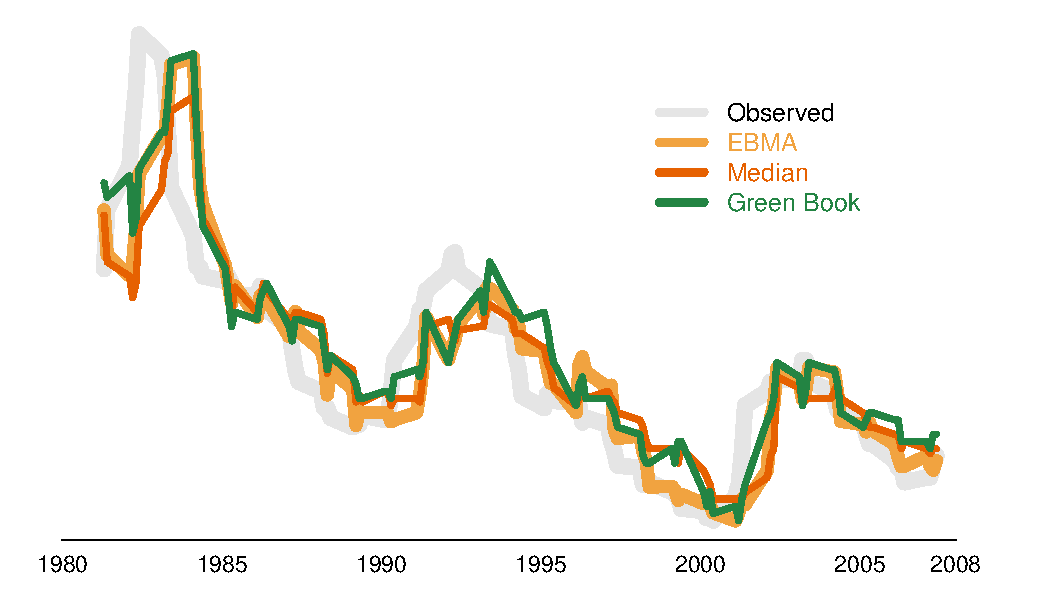
\includegraphics[scale=.8]{mdwtimeSeries2}
\end{center}
\end{figure}


\end{document}



